% Source: https://scnajei2ds6y.feishu.cn/wiki/YJhWwVYCyiqdEMkUsWIcovFun3b
% Faithful Feishu transcription; images are screenshots of normal image preview.
\documentclass[zihao=false,fontset=windows]{ctexart}
% ctexart 不接受任意 pt 选项。正文改 {10pt}，方括号里是行距。
\usepackage{scrextend}
\changefontsizes[12pt]{10pt}

\usepackage[a4paper,left=2.35cm,right=2.35cm,top=1.7cm,bottom=1.9cm]{geometry}
\usepackage{xcolor}
\usepackage{graphicx}
\usepackage{amsmath,amssymb}
\usepackage{enumitem}
\usepackage{tabularx}
\usepackage{colortbl}
\usepackage{listings}
\usepackage{hyperref}
\usepackage[most]{tcolorbox}

\definecolor{feishuText}{RGB}{31,35,41}
\definecolor{feishuBlue}{RGB}{36,91,219}
\definecolor{feishuRed}{RGB}{216,57,49}
\definecolor{feishuGray}{RGB}{100,106,115}
\definecolor{feishuGray2}{RGB}{143,149,158}
\definecolor{feishuPinkBg}{RGB}{251,191,188}
\definecolor{quoteBar}{RGB}{51,112,255}
\definecolor{codebg}{RGB}{245,246,247}
\definecolor{codeborder}{RGB}{222,224,227}
\definecolor{inlinebg}{RGB}{242,243,245}
\definecolor{callRed}{RGB}{253,226,226}
\definecolor{callOrange}{RGB}{255,245,235}
\definecolor{callYellow}{RGB}{254,255,240}
\definecolor{callGreen}{RGB}{240,251,239}
\definecolor{callBlue}{RGB}{240,244,255}
\definecolor{callRedSoft}{RGB}{254,241,241}
\definecolor{callSun}{RGB}{255,255,204}
\definecolor{tableHead}{RGB}{242,243,245}
\definecolor{tableRule}{RGB}{222,224,227}
\definecolor{codeText}{RGB}{31,35,41}
\definecolor{codeKeyword}{RGB}{0,0,255}
\definecolor{codeComment}{RGB}{0,128,0}
\definecolor{codeString}{RGB}{163,21,21}

\setmainfont{Times New Roman}
\setCJKmainfont{Microsoft YaHei}[AutoFakeBold=2.2]
\setCJKsansfont{Microsoft YaHei}[AutoFakeBold=2.2]
\setCJKmonofont{Microsoft YaHei}[AutoFakeBold=2.2]
\setmonofont{Consolas}
\newfontfamily\emojifont{Segoe UI Emoji}

\hypersetup{
  colorlinks=true,
  urlcolor=feishuBlue,
  linkcolor=feishuBlue,
  unicode=true,
  pdftitle={InstructBLIP(2023, Salesforce Research)}
}

\setlength{\parindent}{0pt}
\setlength{\parskip}{0.42em}
\setlength{\fboxsep}{1.5pt}
\setlength{\emergencystretch}{3em}
\linespread{1.28}
\color{feishuText}
\arrayrulecolor{tableRule}
\urlstyle{same}

\setlist[enumerate]{label=\textcolor{feishuBlue}{\arabic*.}, leftmargin=1.7em, itemsep=0.22em, topsep=0.28em, parsep=0.08em, partopsep=0pt}
\setlist[itemize,1]{label=\textcolor{feishuBlue}{\textbullet}, leftmargin=1.35em, itemsep=0.18em, topsep=0.25em, parsep=0.06em, partopsep=0pt}
\setlist[itemize,2]{label=\textcolor{feishuBlue}{◦}, leftmargin=1.45em, itemsep=0.12em, topsep=0.15em}
\setlist[itemize,3]{label=\textcolor{feishuBlue}{\rule[0.18em]{0.38em}{0.38em}}, leftmargin=1.55em, itemsep=0.1em, topsep=0.12em}

\newcommand{\feiEmoji}[1]{{\emojifont #1}}
\newcommand{\incode}[1]{\colorbox{inlinebg}{\ttfamily\small #1}}
\newcommand{\bigmath}[1]{%
  \begin{center}\large$\displaystyle #1$\end{center}%
}

\lstset{
  language=Python,
  basicstyle=\ttfamily\footnotesize\color{codeText},
  keywordstyle=\color{codeKeyword},
  commentstyle=\color{codeComment},
  stringstyle=\color{codeString},
  showstringspaces=false,
  breaklines=true,
  columns=fullflexible,
  keepspaces=true,
  tabsize=4,
  upquote=true,
  aboveskip=2pt,
  belowskip=0pt,
  xleftmargin=0pt,
  frame=none
}

\tcbset{
  feishubase/.style 2 args={
    enhanced,
    boxrule=0pt,
    arc=8pt,
    left=10pt,
    right=10pt,
    top=7pt,
    bottom=7pt,
    before skip=6pt,
    after skip=6pt,
    colback=#1,
    colframe=#1,
    before upper={\feiEmoji{#2}\hspace{0.45em}\ignorespaces}
  }
}
\newtcolorbox{feishubox}[2]{feishubase={#1}{#2}, breakable}
\newtcolorbox{feishuboxnb}[2]{feishubase={#1}{#2}}

\newtcolorbox{feishuquote}{
  enhanced,
  breakable,
  boxrule=0pt,
  leftrule=3pt,
  arc=0pt,
  colframe=quoteBar,
  colback=white,
  left=8pt,
  right=2pt,
  top=2pt,
  bottom=2pt,
  before skip=4pt,
  after skip=4pt,
  before upper=\color{feishuGray}
}

\newtcolorbox{feishucode}{
  enhanced,
  breakable,
  colback=codebg,
  colframe=codeborder,
  boxrule=0.6pt,
  arc=6pt,
  left=6pt,
  right=6pt,
  top=5pt,
  bottom=4pt,
  before skip=6pt,
  after skip=6pt
}

\definecolor{sourceGreenSolid}{HTML}{D9F5D6}
\definecolor{sourceGreenText}{HTML}{2D8F3C}

\begin{document}
{\zihao{1}\bfseries InstructBLIP(2023, Salesforce Research)\par}
\begin{feishuquote}
InstructBLIP：图像上的指令微调（2023.05, Salesforce Research）\par

\href{https://arxiv.org/abs/2305.06500}{InstructBLIP: Towards General-purpose Vision-Language Models with Instruction Tuning}\par

\end{feishuquote}


InstructBLIP 是 BLIP 作者团队在多模态领域的又一续作，基于\textbf{BLIP2}提出了一个\textcolor{feishuRed}{\textbf{视觉-语言的多模态指令微调系统}}，加强了图文对话的能力，并提供系统性的研究来提高模型对未见过的数据和任务的泛化能力，通过统一的自然语言使通用模型能够解决各种视觉语言任务。并且作者经过实验验证，它具有 SOTA 的 zero-shot 能力。\par

InstructBLIP模型\textbf{更擅长「看」、「推理」和「说」}，能够对复杂图像进行理解、推理、描述，还支持多轮对话等任务，甚至在图片解释和推理上表现优于GPT4（一些人认为是因为基于比较强大的BLIP2，才可以「看」的更好）。\par

\par\vspace{1.15em}\noindent{\zihao{-2}\bfseries 1. 背景}\par\vspace{0.28em}
在 NLP 领域，指令微调技术 (Instruction-Tuning) 帮助LLM推广到各种各样的任务上面。\par

\begin{feishuquote}
做法就是对预训练好的大语言模型进行有监督微调，只是这个微调的数据集中包含了很多自然语言指令，指令微调技术使得模型能够处理并遵循人类的指令。\par

\end{feishuquote}
而且通过指令微调得到的LLM已经在多模态模型里面使用了，比如 BLIP-2中的LLM就是。但是这些都是 LLM 领域的指令微调，只被证明了在 NLP 领域的泛化性能不错。\par

由于额外的视觉输入带来了丰富的输入分布和任务多样性，在构建通用的视觉-语言模型上仍具有挑战性。\par

大多数先前的工作大概可以分为下面两种：\par

\begin{tcbraster}[raster columns=2,raster equal height=rows,raster column skip=9pt,raster row skip=8pt,raster left skip=0pt,raster right skip=0pt]
\begin{feishuboxnb}{callGreen}{✨}
多任务学习，将各种视觉语言任务制定相同的输入输出格式。\par

缺点：\textcolor{feishuBlue}{没有经过指令学习的多模态模型泛化能力不佳}\par

\end{feishuboxnb}
\begin{feishuboxnb}{callBlue}{✨}
用额外的视觉组件来扩展预训练LLM，并使用image caption进行训练\par

缺点：\textcolor{feishuBlue}{受限于数据，无法广泛的泛化到需要超出视觉描述的多模态任务}\par

\end{feishuboxnb}


\end{tcbraster}


因此，为了得到一个通用的、统一的视觉语言预训练的多模态模型，作者提出了 InstructBLIP：研究如何在视觉语言任务上进行指令微调，使得训练出的模型可以解决一系列的视觉任务。\par

\begin{feishubox}{callSun}{🌟}
\textcolor{feishuRed}{\textbf{核心点}}：\par

\begin{itemize}
\item \textbf{数据集}：\par
\begin{itemize}
\item 将 26 个数据集转换为指令微调格式，并将它们归类到 11 个任务类别上。使用其中13个数据集（held-in）进行指令微调，并使用 13 个数据集（held-out）和四个完整的任务类别进行 zero-shot 评估。

\item 数据集配比：提出了一种\textbf{平衡采样策略}，以同步不同数据集间的学习进度

\end{itemize}
\item \textbf{模型结构}：\par
提出了一种新的指令感知视觉特征提取机制，能够\textbf{根据输入文本，提取特定的图像特征}。简单来说，\textbf{就是文本不仅输入到LLM，也输入到Q-Former}（\textcolor{feishuBlue}{以此能从冻结的图像编码器中提取指令感知的视觉特征}）\textbf{，Q-Former的输出再又给到LLM}。\par

\item \textbf{使用的预训练模型}：\par
评估和开源了一套 InstructBLIP 模型，它用了两个 LLMs 家族：\par

\begin{itemize}
\item FlanT5：一个基于 Encoder-Decoder Transformer T5 的指令微调LLM模型；

\item Vicuna：一个基于 Decoder LLaMa 的微调LLM模型。

\end{itemize}
InstructBLIP 在广泛的视觉语言任务上实现了最先进的 zero-shot 性能。此外，当 InstructBLIP 模型用作单个下游任务的模型初始化时，可以得到最先进的微调性能。\par

\end{itemize}
\end{feishubox}


为了应对上述挑战，本文提出了一个视觉语言指令调整框架—InstructBLIP，使通用模型能够通过统一的自然语言接口解决各种视觉语言任务。InstructBLIP 使用不同的指令数据集来训练多模态 LLM。具体来说，使用预先训练好的 BLIP-2 模型进行初始化训练，该模型由一个图像编码器、一个 LLM 和一个查询转换器（Q-Former）组成，是二者的桥梁。在指令调整过程中，保持图像编码器和 LLM 不变，对 Q-Former 进行微调。\par



\par\vspace{1.15em}\noindent{\zihao{-2}\bfseries 2. 模型方法}\par\vspace{0.28em}
\par\vspace{0.95em}\noindent{\zihao{3}\bfseries 2.1 数据集}\par\vspace{0.28em}
\par\vspace{0.75em}\noindent{\zihao{4}\bfseries 2.1.1 数据集划分}\par\vspace{0.28em}
为了确保指令微调数据的多样性，作者收集了来自 11 种不同任务的 26 个数据集，并将它们转换为指令调优格式：\par

\begin{feishuquote}
其中包含：图像描述、图像描述与阅读理解、视觉推理、图文问答、基于知识的图像问答、带有阅读理解的图文问答、图像问题生成（与QA问题相反）、视频问答、视觉对话问答、图像分类、LLaVA-Instruct-150K\par

\end{feishuquote}
\begin{center}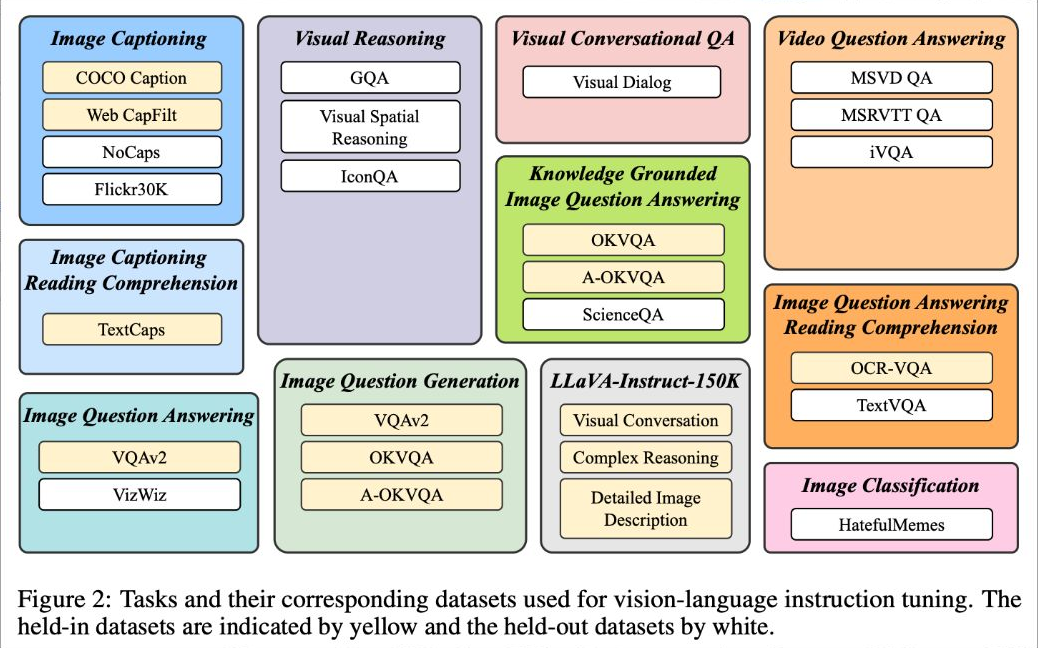
\includegraphics[width=0.98\linewidth]{images/2023-InstructBLIP/fig-01.png}\end{center}
训练集划分：上图中26个数据集中，13个数据集（黄色，held-in data）用于\textbf{Q-Former微调训练}，另外13个数据集（白色，held-out data）用于\textbf{zero-shot能力测试}。\par

\begin{feishuquote}
\textbf{Held-in Data}：用于训练或调优模型的数据。这部分数据是“包含在”模型训练过程中的，可能用于训练（training set）或验证（validation set）。\par

\textbf{Held-out Data}：被“保留在外”的数据，不参与模型训练，而是用于最终评估模型的泛化能力，通常是测试集（test set）。有时，在超参数调整时，特定的一部分数据也可能被作为held-out validation set，以防止数据泄漏。\par

\end{feishuquote}
作者的目标是探究指令微调如何提高模型在没见过的数据集上的 zero-shot 表现，所以在zero-shot测试集中（held-out data）又继续分成两种：\par

\begin{enumerate}
\item[\textcolor{feishuBlue}{1.}] 数据集在训练过程中没有被模型看到过，但同任务类型在训练集中出现，被模型学过，比如视觉问答任务中的VizWiz数据集。\par
\begin{feishuquote}
这种类型的 held-out 数据评估并不简单，因为 held-out 数据集和训练数据集之间存在数据分布的偏移。\par

\end{feishuquote}
\item[\textcolor{feishuBlue}{2.}] 数据不仅在训练期间没有被模型看过，而且同类型的任务也没被模型学过，比如视觉推理、视频问答、视觉对话问答和图像分类任务的数据集。

\end{enumerate}
\textcolor{sourceGreenText}{在训练期间，把所有的 held-in 数据集的训练集混合之后，并在不同任务中均匀采样 instruction templates，使用语言建模损失函数训练模型，即给模型输入图片和 instruction templates，希望它输出回答。}\par

\par\vspace{0.75em}\noindent{\zihao{4}\bfseries 2.1.2 指令模版}\par\vspace{0.28em}
数据集需要转化为图文指令微调的形式，用于多模态大语言模型的训练。\par

\begin{feishuquote}
\feiEmoji{🌰}：在图像分类任务中，图片A的类别是狗，数据的组织形式要转换成：\par

\textcolor{feishuBlue}{\incode{问题：图片A，请问图片的类别是什么}}\par

\textcolor{feishuBlue}{\incode{回答：类别是狗}}\par

\end{feishuquote}
针对不同的任务类型，有多样化模板（10\textasciitilde{}15 个自然语言指令模板）来进行数据的形式转换：\par

\begin{center}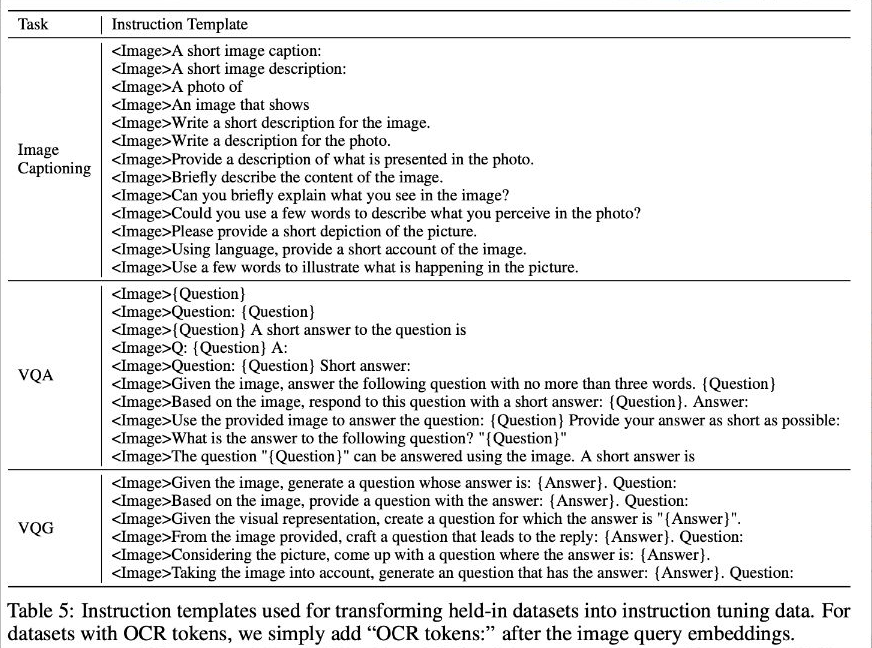
\includegraphics[width=0.98\linewidth]{images/2023-InstructBLIP/fig-02.png}\end{center}
这些模板清晰指出任务和目标，可以分为3类：\par

\begin{itemize}
\item 图像描述\par
\begin{itemize}
\item \feiEmoji{🌰}：“A shot image caption:”“A photo of ”

\item 一共 13 个模板

\end{itemize}
\item 视觉问答\par
\begin{itemize}
\item \feiEmoji{🌰}：“\{直接贴问题\}”、“Q:\{问题\} A:”

\item 一共 10 个模板

\end{itemize}
\item 视觉问题生成\par
\begin{itemize}
\item \feiEmoji{🌰}：“Geven the image，generate a question whose answer is:\{Answer\}. Question:”

\item 一共 6 个模板

\end{itemize}
\end{itemize}

\begin{feishubox}{callOrange}{⚠}
\begin{enumerate}
\item[\textcolor{feishuBlue}{1.}] 对于一些偏向或容易有简短回答的数据集，作者刻意地在 instruction 中添加了\textcolor{feishuBlue}{\incode{short answer}}\textcolor{feishuBlue}{、}\textcolor{feishuBlue}{\incode{as short as possible}}或是\textcolor{feishuBlue}{\incode{briefly}}字样来降低模型过拟合的风险，防止其始终生成很短的输出。（\textcolor{feishuRed}{\textbf{防止过拟合的方式是：在指令中有所体现}}）

\item[\textcolor{feishuBlue}{2.}] 对于LLaVA-Instruct-150K数据集，由于其指令格式是自然结构的，因此无需添加额外的指令模板。

\item[\textcolor{feishuBlue}{3.}] 对于涉及场景文本的数据集，OCR 标记作为补充信息添加到指令中。

\end{enumerate}
\end{feishubox}
\par\vspace{0.75em}\noindent{\zihao{4}\bfseries 2.1.3 均衡训练集}\par\vspace{0.28em}
\feiEmoji{🙋}：由于训练数据集的数量众多，而且每个数据集的大小差异很大，均匀地混合这些数据集可能会导致-->\textcolor{feishuBlue}{模型在小数据集上过拟合，在大数据集上欠拟合}。\par

\feiEmoji{✅}：提出了一种按照数据集大小加权采样的方法。\par

具体采样方法：\par

假设有$D$个数据集，每个数据的大小为$S_1,S_2,...,S_D$，那么第$d$个数据集的采样概率（从该数据集中选取一个训练样本的概率）为：$p_d=\sqrt{S_d}/\displaystyle\sum_{i=1}^{D}\sqrt{S_i}$。\par

同时作者还对某些数据集的权重进行了手动微调，以提高其收敛性。特别是降低了以多选题为特色的 A-OKVQA 的权重，增加了需要生成开放式文本的 OKVQA 的权重。。\par

\begin{feishuquote}
因：数据集和任务之间存在固有的差异，尽管数据集和任务的规模相似，但却需要不同程度的训练强度。\par

\end{feishuquote}


\par\vspace{0.95em}\noindent{\zihao{3}\bfseries 2.2 模型结构\&训练策略}\par\vspace{0.28em}
在当时，像BLIP-2这种现有的零样本图像到文本的生成方法，在提取视觉特征时采取了与指令并无关系的方法。也就是说，LLM中的视觉输入是不知道指令的（\textbf{Instruction-agnostic}），这并不利于该模型在不同任务中的灵活性。\par

因此，如果模型可以适应多个任务类型，将任务类型作为指令信息之一，来产生相关的视觉表征，就能使得模型在任务类型上获得零样本能力。这样的话，相同的输入图像，在不同的\textbf{任务指令}下会有很大的变化。所以，\textcolor{feishuRed}{指令感知的视觉模型可以提高模型从不同指令中学习的能力。}\par

\feiEmoji{🌰} 考虑两种情况：（可以认为这是\textbf{指令调整的优点}\textbf{）}\par

\feiEmoji{1⃣} 输入同一图像，模型被要求完成两个不同的任务 \feiEmoji{➡}\feiEmoji{➡}\textcolor{sourceGreenText}{ 一个指令感知的视觉模型可以根据指令从同一图像中提取不同的特征，在解决不同任务时呈现出更多的信息特征}\par

\feiEmoji{2⃣} 给定两个不同的图像，模型被指示完成同一任务 \feiEmoji{➡}\feiEmoji{➡} \textcolor{sourceGreenText}{一个指令感知的视觉模型可以利用指令中体现的共同知识来提取两个不同图像的特征，从而实现图像之间更好的信息转移}\par



InstructBLIP通过充分使用BLIP-2模型中的Q-Former架构，提出了一种指令感知的视觉特征提取方法。\par

InstructBLIP的模型架构和BLIP-2类似，区别在于输入文本换成了指令数据Instructions，都包含\textbf{图像编码器、Q-Former }和\textbf{ LLM}，并使用预训练的BLIP-2模型进行初始化。\par

\begin{center}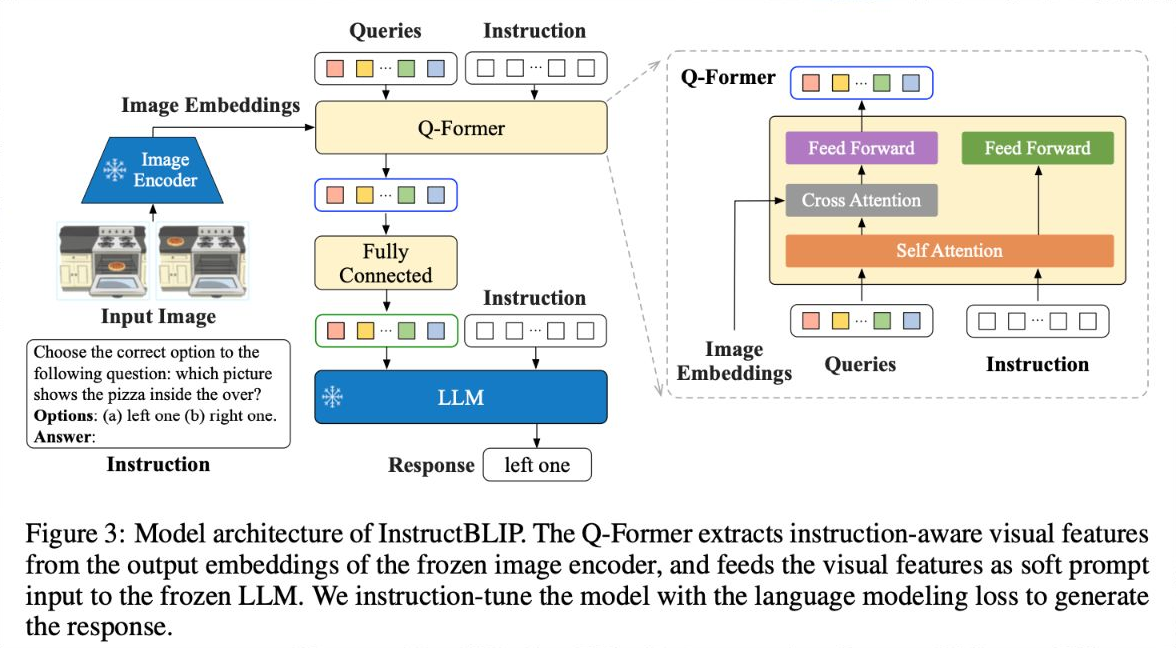
\includegraphics[width=0.98\linewidth]{images/2023-InstructBLIP/fig-03.png}\end{center}
模型的前向过程如下所示：\par

\begin{enumerate}
\item[\textcolor{feishuBlue}{1.}] 输入的图片通过冻结的图像编码器提取图像特征，并输入到 Q-Former 中，此外Q-Former的输入还包括可学习的 Queries (BLIP-2 的做法) 和 Instruction。\par
\begin{feishuquote}
Q-Former的输入：\textcolor{feishuRed}{图像特征 + 可学习的Queries + Instruction}\par

\end{feishuquote}
\item[\textcolor{feishuBlue}{2.}] Q-Former 的内部结构如上图右侧所示，可学习的 Queries 通过 \textcolor{feishuRed}{\textbf{Self-Attention}} 和 Instruction 交互，然后通过 \textcolor{feishuRed}{\textbf{Cross-Attention}} 和输入图片的特征交互，用于提取与 Instruction 相关的图像特征。

\item[\textcolor{feishuBlue}{3.}] Q-Former 的输出通过一个 FC 进行 transform 后送入到冻结的 LLM 中，生成回复。

\end{enumerate}
Q-Former 在指令微调前的预训练过程遵循 BLIP-2 的两步：\par

\begin{enumerate}
\item[\textcolor{feishuBlue}{1.}] 预训练1：首先冻结图像编码器的参数，预训练 Q-Former 的参数，训练目标是视觉语言建模（ITC、MLM、ITM）。使用image caption数据，学习视觉文本相关性表示。

\item[\textcolor{feishuBlue}{2.}] 预训练2：其次冻结 LLM 的参数，预训练 Q-Former 的参数，训练目标是文本生成（LM）。使用image caption数据，学习对齐LLM的文本生成。

\item[\textcolor{feishuBlue}{3.}] 指令微调：在预训练之后，通过指令调整对 Q-Former 进行微调，其中 LLM 接收来自 Q-Former 的视觉编码和任务指令作为输入（\textcolor{feishuBlue}{Q-Former的输出 + Instruction在embedding层面融合，输入到LLM中}）。使用Instruction任务数据，学习遵循指令生成回复的能力。

\end{enumerate}
\begin{feishubox}{callOrange}{⚠}
在InstructBLIP中，指令文本不仅作为输入到了LLM中，同时也输入到了Q-Former中。\par

\textcolor{sourceGreenText}{指令instruction不仅会指导LLM生成文本，同时也会提取不同的视觉特征}\par

\end{feishubox}
指令信息使得Q-Former模型更加关注图像特征中和任务相关的信息。\textcolor{feishuRed}{从prompt的角度来看，图像特征是一种}\textcolor{feishuRed}{\textbf{软提示（soft prompt）}}\textcolor{feishuRed}{，指令是一种相对较“硬”的提示。}\par

\begin{feishubox}{callSun}{🌟}
一句话概括：\par

Q-Former 提取指令感知的图像特征（Instruction-aware vision model），根据指令的不同获取不同的图像特征。然后将这些图像特征作为LLM的软视觉提示（soft prompt），使用LM loss和指令微调模型生成回复。\par

\end{feishubox}
\begin{feishubox}{sourceGreenSolid}{🙋}
\textcolor{feishuBlue}{\textbf{在 InstructBLIP 中，Q-Former 如何根据不同的指令筛选不同的视觉细节？}}\par

在 \textbf{InstructBLIP} 的架构中，Q-Former 的核心作用是作为 \textbf{视觉-语言的桥梁}，它的关键特性是\textbf{动态筛选与指令相关的视觉特征}。\par

\begin{enumerate}
\item[\textcolor{feishuBlue}{1.}] \textbf{Q-Former 通过 Instruction 引导 Queries 的关注区域}\par
在 \textbf{前向传播（Forward Pass）} 中，\textbf{Q-Former 内部处理（关键部分）}：\par

A. \textbf{第一步：Queries + Instruction 通过 Self-Attention 交互}\par
\begin{itemize}
\item Queries 并不是静态的，而是可以自适应地调整它们对图像的关注点。

\item 用户的指令 \textbf{会影响 Queries 的自注意力机制（Self-Attention）}，让它们对不同任务产生不同的搜索偏好。

\end{itemize}
B. \textbf{第二步：Queries 与 图像特征 通过 Cross-Attention 交互}\par
\begin{itemize}
\item Queries 通过 Cross-Attention 从图像特征中提取 \textbf{与 Instruction 相关的视觉信息}，而不是盲目读取所有图像信息。

\item \textbf{不同的 Instruction 会改变 Queries 的关注点}：\par
\begin{itemize}
\item “这是什么动物？” → Queries 关注整体形状和轮廓。

\item “它的眼睛是什么颜色？” → Queries 关注局部区域（眼睛）。

\item “背景里有什么？” → Queries 关注背景，而忽略主体。

\end{itemize}
\end{itemize}
\item[\textcolor{feishuBlue}{2.}] \textbf{训练过程：确保 Q-Former 学会“选择”合适的视觉信息}\par
Q-Former 的训练策略保证了：\par

\begin{itemize}
\item Q-Former 既不会把所有图像信息都传给 LLM（避免冗余），也不会遗漏关键细节（提升任务相关性）。

\item 指令不同，Q-Former 选择的信息就不同，使模型具有高度的指令适应能力。

\end{itemize}
\end{enumerate}
\textcolor{feishuBlue}{Q-Former 能够根据指令选择不同的视觉细节，主要依赖于：}\par

\begin{itemize}
\item \textcolor{feishuBlue}{\textbf{Self-Attention 使 Queries 理解指令，Cross-Attention 让 Queries 选择相关图像特征。}}

\item \textcolor{feishuBlue}{\textbf{通过两阶段训练，Q-Former 学会根据不同指令自动筛选关键信息，而非盲目传递所有图像信息。}}

\item \textcolor{feishuBlue}{\textbf{LLM 仅接受经过 Q-Former 处理后的视觉特征，从而根据用户指令生成合理的回答。}}

\end{itemize}
\end{feishubox}
训练细节：\par



\begin{feishucode}
\begin{lstlisting}
@registry.register_model("blip2_vicuna_instruct")
class Blip2VicunaInstruct(Blip2Base):
    """
    BLIP2 Vicuna 模型。
    支持的模型类型:
        - vicuna7b
        - vicuna13b
    用法示例:
        >>> from lavis.models import load_model
        >>> model = load_model("blip2_vicuna_instruct", "vicuna7b")
    """

    ......
    
    def __init__(
        self,
        vit_model="eva_clip_g",           # vision encoder 模型名称
        img_size=224,                     # 输入图像尺寸
        drop_path_rate=0,                 # DropPath 的比率
        use_grad_checkpoint=False,        # 是否使用梯度检查点，以节省显存
        vit_precision="fp16",            # vision encoder 的精度
        freeze_vit=True,                  # 是否冻结 vision encoder 的参数
        num_query_token=32,              # Q-former 的可学习查询 token 数量
        llm_model="",                     # LLM（Vicuna）的检查点路径或名称
        prompt="",                        # 默认提示语字符串
        max_txt_len=128,                  # 输入文本的最大长度
        max_output_txt_len=256,           # 生成文本的最大长度
        apply_lemmatizer=False,           # 是否在推理后对文本进行词形还原
        qformer_text_input=True,          # Q-former 是否接收文本输入
    ):
        
        ......
        
        # 是否冻结视觉编码器
        if freeze_vit:
            for name, param in self.visual_encoder.named_parameters():
                param.requires_grad = False
            self.visual_encoder = self.visual_encoder.eval()
            self.visual_encoder.train = disabled_train  # 禁用训练
            logging.info("freeze vision encoder")

        # 初始化 Q-former 模块以及可学习的查询 token
        self.Qformer, self.query_tokens = self.init_Qformer(
            num_query_token, self.visual_encoder.num_features
        )

        # 如果不需要 Q-former 的文本输入，则把对应的层置为 None
        if not qformer_text_input:
            self.Qformer.bert.embeddings.word_embeddings = None
            self.Qformer.bert.embeddings.position_embeddings = None
            for layer in self.Qformer.bert.encoder.layer:
                layer.output = None
                layer.intermediate = None
        else:
            # 如果需要文本输入，就调整 Q-former 的词表大小以适配 tokenizer
            self.Qformer.resize_token_embeddings(len(self.tokenizer))
        self.Qformer.cls = None  # 不需要分类头

        # 初始化 Llama tokenizer
        self.llm_tokenizer = LlamaTokenizer.from_pretrained(llm_model, use_fast=False, truncation_side="left")
        # 从预训练权重中加载 LlamaForCausalLM 模型
        self.llm_model = LlamaForCausalLM.from_pretrained(
            llm_model, torch_dtype=torch.float16
        )
        
        ......

        # 重新 resize LLM 的词嵌入（embedding）层大小，以匹配添加了新 token 的 tokenizer
        self.llm_model.resize_token_embeddings(len(self.llm_tokenizer))

        # 下面是另一种获取 eos_token_id 的方法，这里被注释了
        # self.eos_token_id = self.llm_tokenizer(
        #     self.llm_tokenizer.eos_token, add_special_tokens=False
        # ).input_ids[0]

        # 冻结 LLM 参数，使其不可训练
        for name, param in self.llm_model.named_parameters():
            param.requires_grad = False

        # 线性投影层，用于将 Q-former 输出向量映射到 LLM 的隐藏维度
        self.llm_proj = nn.Linear(
            self.Qformer.config.hidden_size, self.llm_model.config.hidden_size
        )

        ......

        self.qformer_text_input = qformer_text_input  # 是否在 Q-former 阶段允许文本输入

    def concat_text_input_output(self, input_ids, input_atts, output_ids, output_atts):
        """
        将文本输入与输出拼接到一起，供 LLM 做统一的训练（即在顺序上：输入 + 输出 + 输入剩余部分）。
        """
        
        ......
        
        return llm_tokens, input_part_targets_len

    def forward(self, samples):
        """
        前向传播，用于训练阶段（有监督训练）。
        接收 samples，其中包括图像和文本（输入/输出）等内容。
        """
        # image 是输入图像数据
        image = samples["image"]
        with self.maybe_autocast():
            # 用视觉编码器得到图像特征
            image_embeds = self.ln_vision(self.visual_encoder(image))
        # 构建图像特征的 attention mask，全是 1
        image_atts = torch.ones(image_embeds.size()[:-1], dtype=torch.long).to(image.device)

        bs = image.size(0)  # batch size

        # 将可学习查询 token 扩展成 batch 数量
        query_tokens = self.query_tokens.expand(image_embeds.shape[0], -1, -1)
        # 如果在 Q-former 中需要文本输入
        if self.qformer_text_input:
            # 利用 tokenizer 对 samples["text_input"] 进行处理
            text_Qformer = self.tokenizer(
                samples["text_input"],
                padding='longest',
                truncation=True,
                max_length=self.max_txt_len,
                return_tensors="pt",
            ).to(image.device)
            # 对查询 token 的 attention mask 也全为 1
            query_atts = torch.ones(query_tokens.size()[:-1], dtype=torch.long).to(image.device)
            # 将两部分的 atts 拼接
            Qformer_atts = torch.cat([query_atts, text_Qformer.attention_mask],dim=1)

            # 送入 Q-former 的 bert
            query_output = self.Qformer.bert(
                text_Qformer.input_ids,
                attention_mask=Qformer_atts,
                query_embeds=query_tokens,
                encoder_hidden_states=image_embeds,
                encoder_attention_mask=image_atts,
                return_dict=True,
            )
        else:
            # 不带文本输入的 Q-former
            query_output = self.Qformer.bert(
                query_embeds=query_tokens,
                encoder_hidden_states=image_embeds,
                encoder_attention_mask=image_atts,
                return_dict=True,
            )

        # 只取查询 token 对应的输出部分，并通过线性层映射到 LLM 的隐藏维度
        inputs_llm = self.llm_proj(query_output.last_hidden_state[:,:query_tokens.size(1),:])
        # 对应的 attention 全部为 1
        atts_llm = torch.ones(inputs_llm.size()[:-1], dtype=torch.long).to(image.device)

        # LLM 的 tokenizer；生成输入 tokens
        self.llm_tokenizer.padding_side = "right"
        self.llm_tokenizer.truncation_side = 'left'
        text_input_tokens = self.llm_tokenizer(
            samples['text_input'],
            return_tensors="pt",
            padding="longest",
            truncation=True,
            max_length=self.max_txt_len,
        ).to(image.device)

        # 输出文本 tokens（也就是标签）
        self.llm_tokenizer.truncation_side = 'right'
        text_output_tokens = self.llm_tokenizer(
            [t + self.llm_tokenizer.eos_token for t in samples['text_output']],
            return_tensors="pt",
            padding="longest",
            truncation=True,
            max_length=self.max_output_txt_len,
        ).to(image.device)

        # 将输入与输出拼接，以得到真正送入 LLM 的内容
        llm_tokens, input_part_targets_len = self.concat_text_input_output(
            text_input_tokens.input_ids,
            text_input_tokens.attention_mask,
            text_output_tokens.input_ids,
            text_output_tokens.attention_mask,
        )

        ......

        # 将 LLM embedding 与 tokens 拼接
        inputs_embeds = self.llm_model.get_input_embeddings()(llm_tokens['input_ids'])
        inputs_embeds = torch.cat([inputs_llm, inputs_embeds], dim=1)
        # 同步拼接 attention mask
        attention_mask = torch.cat([atts_llm, llm_tokens['attention_mask']], dim=1)

        # 最后传给 LLM 做因果语言建模训练
        with self.maybe_autocast():
            outputs = self.llm_model(
                inputs_embeds=inputs_embeds,
                attention_mask=attention_mask,
                return_dict=True,
                labels=targets,
            )

        loss = outputs.loss  # 计算出的 loss

        return {"loss": loss}  # 返回一个字典格式，包含 loss

    @torch.no_grad()
    def generate(
        self,
        samples,
        use_nucleus_sampling=False,  # 是否使用核采样
        num_beams=5,                 # beam search 的大小
        max_length=256,              # 生成的最大长度
        min_length=1,                # 生成的最小长度
        top_p=0.9,                   # nucleus sampling 的阈值
        repetition_penalty=1.5,      # 重复惩罚系数
        length_penalty=1,            # 长度惩罚系数
        num_captions=1,              # 生成的序列个数
        temperature=1,               # 温度系数
    ):
        """
        推理模式下的文本生成函数。
        """

        self.llm_tokenizer.padding_side = "left"

        # 如果 samples 中包含 "prompt"，就用它，否则用初始化时给定的 self.prompt
        if "prompt" in samples.keys():
            prompt = samples["prompt"]
        else:
            prompt = self.prompt

        ......

        # 如果有 OCR tokens，且 prompt 中包含 "{}"，就把 OCR tokens 替换进去（针对某些文本任务）
        if "ocr_tokens" in samples.keys() and "{}" in prompt[0]:
            prompt = [p.format(', '.join(samples['ocr_tokens'][i][:30])) for i, p in enumerate(prompt)]

        ......
        
        # 针对视频输入（5 维张量，形状 [B, C, T, H, W]）
        if image.dim() == 5:
            ......
        else:
            # 普通情况（单帧图像）
            ......

        # 对 prompt 做 LLM tokenizer
        llm_tokens = self.llm_tokenizer(
            prompt,
            padding="longest",
            return_tensors="pt"
        ).to(image.device)

        # 在自动混合精度下，获取 LLM 的输入嵌入，并与图像查询部分拼起来
        with self.maybe_autocast():
            inputs_embeds = self.llm_model.get_input_embeddings()(llm_tokens.input_ids)
            inputs_embeds = torch.cat([inputs_llm, inputs_embeds], dim=1)
            attention_mask = torch.cat([atts_llm, llm_tokens.attention_mask], dim=1)

            # 使用 HuggingFace 的 generate 函数进行文本生成
            outputs = self.llm_model.generate(
               ......
            )

        ......

        return output_text
\end{lstlisting}
\end{feishucode}
作者重写了bert embedding层的代码，将query\_embeds（可理解为Q-Former的输出）和embeddings（可理解为Instruction的文本embedding） concat起来\par



\par\vspace{1.15em}\noindent{\zihao{-2}\bfseries 3. 推理任务}\par\vspace{0.28em}
对于不同的任务类别，采用不同的推理策略。\par

\feiEmoji{🌰}：\par

\begin{itemize}
\item 对于大部分描述性任务，如 image captioning，open-ended VQA 等，InstructBLIP 可以直接使用 LLM 生成的文本作为输出（\textcolor{feishuBlue}{采用传统的transformer解码方式生成回答}）。

\item 对于选择性任务，如 classification 和 multi-choice VQA等这种回复内容受限的任务 ，InstructBLIP 遵循 ALBEF 的做法生成固定的几种答案，根据概率选择最后的结果作为输出。实际上就是 vocabulary ranking method，将 LLM 生成的内容词汇限制为候选列表进行排序（\textcolor{feishuBlue}{将词汇量限制在候选列表中}），计算每个候选的对数似然，选择数值最大的一个作为最终预测。这种排序方法适用于 ScienceQA、IconQA、A-OKVQA（多选）、HatefulMemes、Visual Dialog、MSVD 和 MSRVTT 数据集 。

\end{itemize}


\end{document}
